\documentclass[11pt]{amsart}
\usepackage{geometry}                % See geometry.pdf to learn the layout options. There are lots.
\geometry{letterpaper}                   % ... or a4paper or a5paper or ... 
%\geometry{landscape}                % Activate for for rotated page geometry
%\usepackage[parfill]{parskip}    % Activate to begin paragraphs with an empty line rather than an indent
\usepackage{graphicx}
\usepackage{amssymb}
\usepackage{epstopdf}
\usepackage{enumerate}
\DeclareGraphicsRule{.tif}{png}{.png}{`convert #1 `dirname #1`/`basename #1 .tif`.png}
\setlength{\parindent}{0in} % no paragraph indent

\usepackage{fancyhdr}
\pagestyle{fancy}
\lhead{\footnotesize \parbox{11cm}{The Effect of the NSA Leaks on Tech Stock Volatility} }
\rhead{\footnotesize \parbox{5cm}{Max Scheiber and Ruslan Zagatskiy} }

\title{The Effect of the NSA Leaks on Tech Stock Volatility - Max Scheiber and Ruslan Zagatskiy}
\date{12.16.2013}

\begin{document}
\maketitle
\section{Abstract}
The NSA scandal of the summer of 2013 changed the way that many Americans viewed the relationship between government and citizens. However, these changes were not strongly reflected in the stock market in either the short or the long run. One of Snowden's leaks briefly spiked volatility, but we do not see any other changes in returns volatility or in trading volume in the securities of the specific tech companies that the NSA had these data agreements with. \\

\section{Introduction}
On June 6th, 2013, Edward Snowden revealed through the British newspaper, \textit{The Guardian}, that the National Security Agency (NSA) can easily extract personal customer data from America's largest tech companies, spanning from email to audio chats. More NSA leaks were released throughout summer 2013. These events fundamentally changed the socioeconomic and political climates of the United States of America. However, did these leaks change the volatility of relevant tech stocks in either the short term or long run? \\

Examining the effect of these leaks on the stock market requires an event-driven approach. A standard way to consider specific date ranges quantitatively is to create a dummy indicator variable for any date that we think is important. Statisticians can perform then use the aforementioned indicator variable as an input to any statistical model, such as a linear regression or a time series model. As Savickas wrote in 2003, \\

\textit{I use a GARCH(1,1) model with dummy variables to evaluate a simple test statistic that accounts for the stochastic behavior of volatility during both event and nonevent periods. The test does not require the volatility effect to be the same across firms in the sample. The test is easy to implement but has substantially higher rejection rates of a false null hypothesis than do the previous tests.} \\

This tests for whether or not there is a time series effect in volatility of any sort - in other words, if volatility is constant throughout a time period or not. A chunk of our analysis uses a very similar model. One thing that is important to note is that this model can show significance, but it is very hard to draw causation. \\

We obtained consolidated trade data from Wharton Research Data Services (WRDS) for Google (GOOG), Apple (AAPL), Microsoft (MSFT), and Facebook (FB) for the January 1st, 2013 through July 31st, 2013 timespan. These consolidated datasets contain average execution prices and total shares volume a few times each second. We chose these stocks because they were the ones identified in the NSA's leaked slide deck. \\

To make data analysis more manageable, we converted this data into hourly buckets from 9am to 3pm, inclusive. We did this by taking the average execution price over each bucket, equally weighted within the bucket. (For the final presentation, it may be better to volume-weight this mean). We also took volume sums for each bucket. \\

We then created a basket of tech stocks by taking the equal-weighted average of each bucket of all stocks considered. The reason for doing this was to enhance our signal-to-noise ratio; this basket would minimize the effects in securities pricing and volatility of, say, one company's earnings report, while confirming sector-wide trends. \\

Within this basket, we computed percent returns, which allowed us to compute a scale-independent moving volatility. We use squared returns as a measure of volatility because they are roughly center around zero. We also measure volatility from a given time bucket over the previous 30 time buckets. Given that there are seven buckets per day, we see our volatility measure cover a duration of just over four days. All analysis in this paper is performed with both measures. \\

\section{Methods}
We explored three main dates. The original leaks happened on \textbf{June 6th, 2013}. \textit{The Guardian} released a second set of leaks on \textbf{June 20th}, and they published a video interview with Snowden on \textbf{July 8th}. \\

We first ran a $GARCH(1,1)$ over the entire data set, which confirmed that the tech sector had heteroskedastic returns over the period. This makes intuitive sense; the stock market probably will have a few days of abnormal trading over a seven-month span. \\

\newpage

\centerline{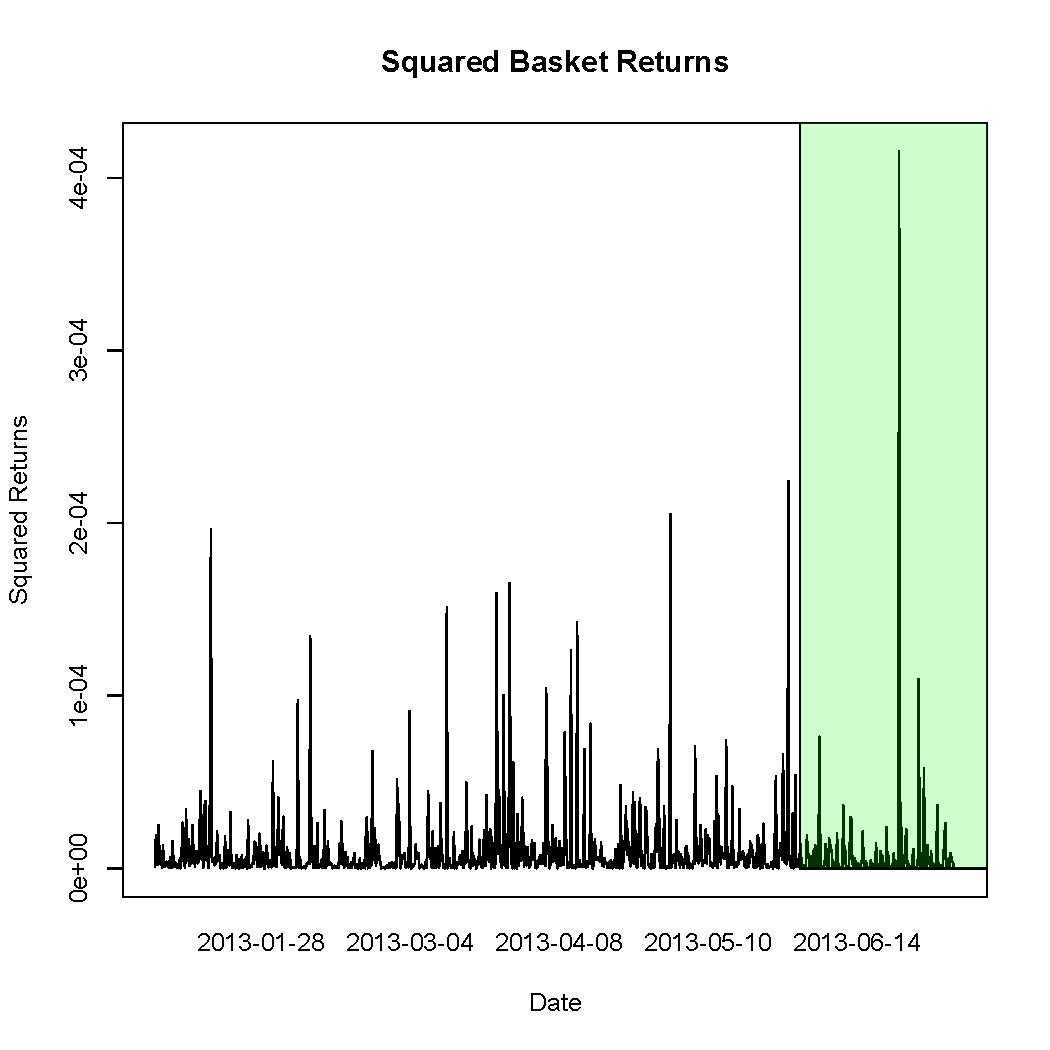
\includegraphics[scale=0.5]{basket_sq_returns_12_08.pdf}}

We next examine the month of June. June by itself has heteroskedastic returns, confirmed by another $GARCH(1,1)$. We next fit an OLS regression with indicator variables for June 6-8 and June 20-22, two of our dates of interest. Only the change in volatility during June 20-22 was statistically significant - and only in the short term (June), not medium term (June-July) or long term (January-July).This holds for both squared returns and the moving volatility model. \\

Moreover, we confirmed this analysis by using trade volume instead of trade returns. Trade volume is heteroskedastic by the $GARCH(1,1)$ and significant on the June 20-22 date range. \\

We see a huge spike in volatility around July 20th, but this doesn't correspond with any NSA news. It's likely from quarterly earnings reports - GOOG and MSFT on the 18th, AAPL and FB on the 24th. The same event-driven models used in previous parts of the paper obviously show that this is significant, but we have no choice but to dismiss that part of July. Dropping an indicator onto the July 8th date range is not significant with our models. Again, we confirm this with moving volatility and with trade volume. \\

\centerline{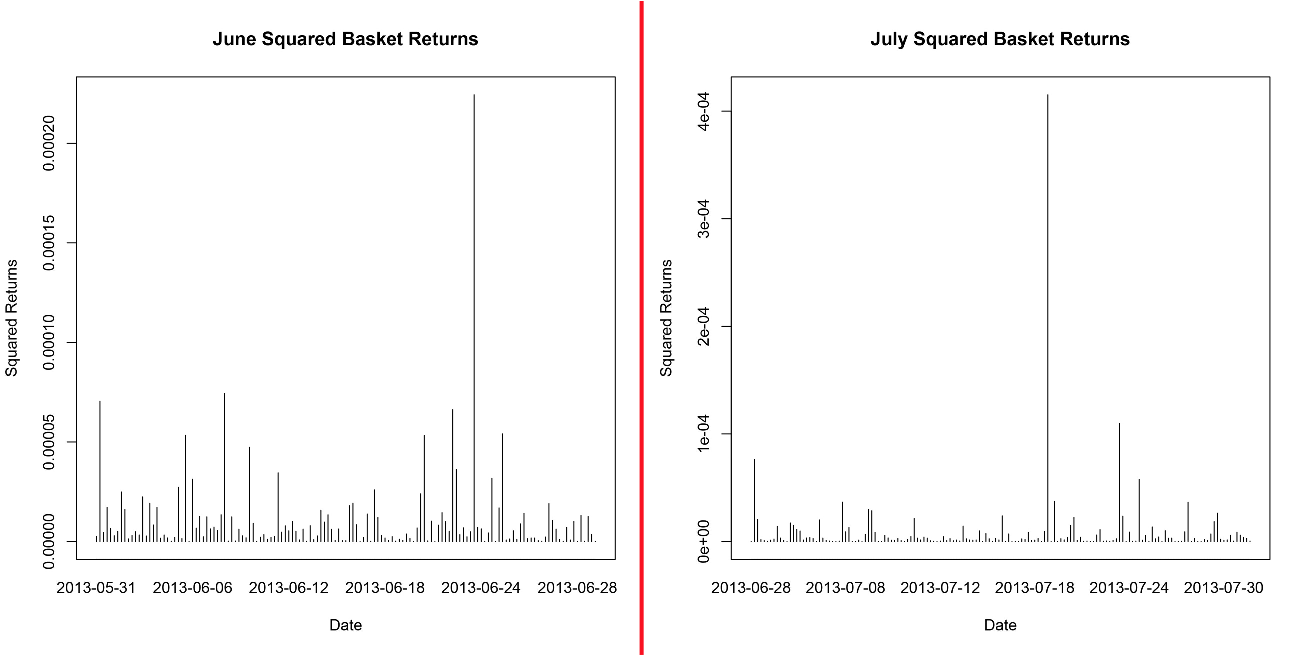
\includegraphics[scale=0.7]{june+july_squared_ret.pdf}}

To get a better sense of the American economic climate at the time, we looked into other large events that would have affected the general stock market at the time. Around June 20th, the only large event was the NSA leak. The Federal Reserve had made an announcement regarding its bond buyback program, but we felt that was minor in comparison to other Fed announcements. Our basis of comparison was that June 20th had one of the three largest spikes in volatility throughout all of 2013 for the VIX, the S\&P 500's exchange-traded fund. \\

\section{Conclusions}
Event-driven analysis is hard to draw conclusions from because it is difficult to untangle correlation from causation. While the statistical analysis we performed was sound, the qualitative analysis performed is not rock-solid. It is hard to avoid confirmation bias when performing qualitative event analysis. We specifically set our dates of concern before even looking at data to avoid being biased in that way, but confirmation bias may have crept in while investigating whether the June 20th volatility spike was caused by something other than the NSA leak. \\

If the NSA leaks have changed how we view the world, the market doesn't really reflect that. There was increased volatility in response to one of the leaks, which may have just been some large institutional investor unloading shares. Moreover, this volatility only persisted for a couple of days. Given that our qualitative analysis is sound, \textbf{the NSA leaks affected short-term volatility in one instance but had no long-term effect whatsoever.} Moreover, any change in volatility that \textit{did} happen affected the entire market, not just tech stocks. \\

\newpage
\section{Appendix}
\end{document}